\documentclass[12pt]{article}

% -------------------------------------------------
% PAGE & LANGUAGE
% -------------------------------------------------

\usepackage[a4paper,margin=2cm]{geometry}

% -------------------------------------------------
% MATHEMATICS
% -------------------------------------------------

\usepackage{amsmath}
\usepackage{amssymb}
\usepackage{amsthm}
\usepackage{mathtools}
\usepackage{yhmath}

% Physics notation
\usepackage{physics}

% -------------------------------------------------
% GRAPHICS & PLOTS
% -------------------------------------------------

\usepackage{graphicx}
\usepackage{tikz}
\usetikzlibrary{patterns}
\usepackage{pgfplots}

\pgfplotsset{compat=1.18}
\graphicspath{{./images/}}

% -------------------------------------------------
% COLORS & BOXES
% -------------------------------------------------

\usepackage[dvipsnames,svgnames,x11names]{xcolor}
\usepackage{tcolorbox}
\tcbuselibrary{skins,breakable}
\newtcolorbox{demobox}[1][]{
    enhanced,
    breakable,
    colback=black!2,
    colframe=black!70,
    boxrule=0pt,
    borderline west={2pt}{0pt}{black!70},
    sharp corners,
    left=10pt,
    right=7pt,
    top=6pt,
    bottom=6pt,
    fonttitle=\bfseries,
    title={Demostració},
    #1
}

\newtcolorbox{examplebox}[1]{
    enhanced,
    breakable,
    colback=black!1,
    colframe=black!15,
    boxrule=0.5pt,
    arc=2mm,
    borderline west={2pt}{0pt}{black!55},
    left=12pt,
    right=12pt,
    top=10pt,
    bottom=10pt,
    before skip=12pt,
    after skip=12pt,
    title={\textbf{Exemple #1}},
    fonttitle=\normalsize,
    coltitle=black,
    attach boxed title to top left={
        xshift=8pt,
        yshift=-\tcboxedtitleheight/2
    },
    boxed title style={
        colback=white,
        colframe=white,
        boxrule=0pt,
        left=3pt,
        right=3pt,
        top=1pt,
        bottom=1pt
    },
    before upper={\setlength{\parskip}{7pt}}
}

% -------------------------------------------------
% DOCUMENT FORMATTING
% -------------------------------------------------

\usepackage{enumitem}
\usepackage[expansion=false]{microtype}
\usepackage{booktabs}
\usepackage{float}
\usepackage{ragged2e}

% -------------------------------------------------
% CHEMISTRY
% -------------------------------------------------

\usepackage[version=4]{mhchem}

% -------------------------------------------------
% LINKS
% --------------------------------------------------

\usepackage[colorlinks=true,linkcolor=Black,urlcolor=Black,citecolor=Black]{hyperref}
\usepackage{tocloft}
\usepackage{cite}

% -------------------------------------------------
% CUSTOM COMMANDS
% -------------------------------------------------

\newcommand{\R}{\mathbb{R}}
\newcommand{\N}{\mathbb{N}}
\newcommand{\Z}{\mathbb{Z}}
\newcommand{\Q}{\mathbb{Q}}

% -------------------------------------------------
% DOCUMENT STYLE
% -------------------------------------------------

\linespread{1.25}

\setlength{\parskip}{0.8em}
\setlength{\parindent}{0pt}

\setlength{\heavyrulewidth}{0.4pt}
\setlength{\heavyrulewidth}{0.4pt}
\setlength{\lightrulewidth}{0.4pt}
\setlength{\cmidrulewidth}{0.4pt}

\title{\textbf{Apunts Càlcul en una Variable}}
\author{\textit{Gerard Cosp Lores}}
\date{\today}

% -------------------------------------------------
% TABLE OF CONTENTS
% -------------------------------------------------

\renewcommand{\contentsname}{Índex}

% Title
\renewcommand{\cfttoctitlefont}{%
    \Huge\bfseries\color{Black}
}

% Line underneath title
\renewcommand{\cftaftertoctitle}{%
    \par\vspace{0.3cm}
    \noindent\color{Black}\rule{\textwidth}{1.2pt}
    \vspace{0.4cm}
}

% Section appearance
\renewcommand{\cftsecfont}{%
    \large\bfseries\color{Black}
}

\renewcommand{\cftsecpagefont}{%
    \large\bfseries\color{Black}
}

% Subsection appearance
\renewcommand{\cftsubsecfont}{%
    \normalsize
}

\renewcommand{\cftsubsecpagefont}{%
    \normalsize\color{Black}
}

% Spacing
\setlength{\cftbeforesecskip}{10pt}
\setlength{\cftbeforesubsecskip}{3pt}

% Dotted leaders
\renewcommand{\cftsecleader}{%
    \color{Black}\cftdotfill{\cftdotsep}
}

\renewcommand{\cftsubsecleader}{%
    \color{Black}\cftdotfill{\cftdotsep}
}

% Number spacing
\setlength{\cftsecnumwidth}{2.5em}
\setlength{\cftsubsecnumwidth}{3.5em}

% -------------------------------------------------

\begin{document}
\justifying

\maketitle
\tableofcontents

\newpage

\section{Nombres \texorpdfstring{$\R$}{R}}

Tenim diferents conjunts de Nombres;

\begin{itemize}
    \item $\N$: Naturals, $\{1,2,3 \dots\}$
    \item $\Z$: Enters, $\{\dots -2,-1,0,1,2 \dots\}$
    \item $Q$: Racionals $\leftrightarrow \{\frac{n}{m}\}$ on $n,m \in \Z - 0$, (tenir en compte que: \textbf{racional - racional = racional} i \textbf{racional/racional = racional}) més d'una fracció pot representar el mateix nombre racional (les anomenem \textit{fraccions equivalents} $\frac{1}{2} = \frac{2}{4}$)
    
    Una fracció pot ser:
    \begin{itemize}
        \item Finita (0.5) on per transformar en fracció \textbf{multipliquem i dividim} per la potència de 10 necessaria
        \item Periòdica (0.4545...) on fem servir un simple truc tal que;
        \begin{equation}
            \begin{aligned}
                0.\wideparen{45} &= y \\
                45.\wideparen{45} &= 100y\\
                45 &= 99y\\
                y &= \frac{45}{99}
            \end{aligned}
        \end{equation}
    \end{itemize}

    \item $\R$: Reals, tots els nombres + els que tenen \textbf{decimals arbitràris} com $\{\pi, e, \sqrt{2}\}$
\end{itemize}

Necessitem el conjunt $\R$, ja que els nombres irracionals no els podem obtenir d'una \textbf{fracció} com és $\frac{n}{m}$

\begin{demobox}
    Si volem demostrar perque $\sqrt{2}$ és irracional, podem demostrar per l'absurd (dir el contrari).
    \begin{align*}
        q &= \sqrt{2} = \frac{n}{m} \\
        q^2 &= 2 = (\frac{n}{m})^2\\
        n^2 &= 2m^2 (parell)\\
        \frac{1}{2}n^2 (parell) &= m^2
    \end{align*}
    com que n i m són parells la fracció $\frac{n}{m}$ és reduïble per 2 per tant ens hem equivocat en el principi i $\sqrt{2}$ ha de ser irracional.
\end{demobox}

\subsection{Conjunts de Nombres}

$A \subset B \rightarrowtail$ Subconjunt pròpi

$A \subseteq B$ És un subconjunt qualsevol i conté B 

x + y ($\in \R$)
Propietats de $\R$
\begin{itemize}
    \item \textbf{Suma}
    \begin{itemize}
        \item Associativa, $(x + y) + z = x + (y + z)$
        \item Commutativa, $x + y = y + x$
        \item Element Neutre, $\exists 0 \in \R \mid x + 0 = 0 + x = x$
        \item Element Simètric, $\forall x \in \R \exists - x \in \R \mid x + (-x) = (-x) + x = 0$ (És l'element neutre)
    \end{itemize}
    \item \textbf{Multiplicació}
    \begin{itemize}
        \item Associativa, $(x\cdot y) \cdot z = x \cdot (y \cdot z)$
        \item Commutativa, $x \cdot y = y \cdot x$
        \item Distributiva, $x \cdot (y + z) = x\cdot y + x\cdot z$
        \item Element Neutre, $\exists 1 \in \R \mid x \cdot 1 = 1 \cdot x = x$
        \item Element Simètric, $\forall x \in \R \exists x^-1 \in \R \mid x \cdot (x^-1) = (x^-1) \cdot x = 1$ (És l'element neutre)
    \end{itemize}
\end{itemize}

\subsection{Valor Absolut}

Definim el valor absolut d'un nombre $\abs{x} \geq 0, \forall x \in \R$.

També podem definir le valor al valor com a;
\[
|x|=
\begin{cases}
 x, & \text{si } x\geq 0\\[4pt]
 -x, & \text{si } x<0
\end{cases}
\]

Ens diu com un nombre \textbf{és més gran independent del signe}, és dir la seva llargada en la recta numérica. $\abs{\pi - 3,14} < 0,01$

Les propietats del valor absolut són les següents;

\begin{itemize}
    \item $\abs{x} \geq 0$
    \item $\text{Si} \abs{x} = 0 \therefore x = 0$
    \item $\abs{x\cdot y} = \abs{x} \cdot \abs{y}$
    \item $\abs{x+y} \neq \abs{x} + \abs{y}$
    \item $\abs{x} \leq y / -y \leq x \leq y $
\end{itemize}

\section{Inducció Matemàtica}

Per poder comprovar que una declaració serveix $\forall x \in \R$ fem servir \textbf{L'inducció matemàtica}. Aquesta té dos condicions que s'han de complir per poder ser cert en tot $\R$

\begin{itemize}
    \item P(1) $\exists$
    \item P(n) $\exists \xRightarrow{}$ P(n+1) $\exists$
\end{itemize}

I això ho podem comprovar per exemple:

\begin{examplebox}{1}

    Si sumem els primers \(n\) nombres obtenim

    \[ 1+2+3+\dots+n=\frac{n(n+1)}{2}. \]

    Per comprovar si aquesta fórmula \(P(n)\) és certa, fem inducció matemàtica.

    \textbf{1. Cas base:}

    \[ P(1)=\frac{1(1+1)}{2}=1. \]

    Per tant, la fórmula és certa per a \(n=1\).

    \textbf{2. Pas inductiu:}

    Suposem que \(P(n)\) és certa:

    \[ P(n)=\frac{n(n+1)}{2}. \]

    Hem de demostrar que també és certa per a \(n+1\):

    \[ P(n+1)=P(n)+(n+1). \]

    Substituïm \(P(n)\):

    \[ P(n+1) = \frac{n(n+1)}{2}+(n+1). \]

    Posem-ho al mateix denominador:

    \[ P(n+1) = \frac{n(n+1)+2(n+1)}{2} = \frac{(n+1)(n+2)}{2}. \]

    Per tant, \(P(n+1)\) també és certa.

    \[ \boxed{P(n)\text{ és certa per a tot }n\geq1.} \]

\end{examplebox}

\begin{examplebox}{2}
    Si tenim la serie

    \[ 1 + 3 + 5 \dots + (2n-1) = n^2 \]

    I volem comprovar que $P(n) = n^2$ és cert fem el mateix d'abans 

    \textbf{1. Cas base:}

    \[ P(1)=1^2 = 1 \]

    Per tant la formùla en 1 és certa ja que $1 = 1$

    \textbf{2. Pas inductiu:}

    Suposem que $P(n)$ és cert:

    \[ P(2n -1 ) = n^2 \]

    Hem de demostrar que també és cert per a $(2n - 1) + 1$

    \[ (2n-1)^2 = (2n-1)^2 + (2n -1 + 1) \]
\end{examplebox}

% inequacions amb inducció

\section{Igualtats}

Anomenem igualtats a un \textit{"statement"} que formulem cert, de manera que $1+1=2$ i sabem que els dos bàndols són idèntics. Ara ens podem preguntar amb quins valor de algun nombre $x$ és cert un statement, de manera que $1+x = 2$ trivialment sabem que $x = 1$ però quan es complica no ho podem fer de cap, \textbf{hem d'aplicar transformacions lineals a tota l'equació}.

Per exemple, si s'ens dona $2x+3 = 0$,

\begin{itemize}
    \item Sumem l'element simètric a $3$, $2x = -3$
    \item Dividim per l'element simètric de $2$, $x = \frac{-3}{2}$
\end{itemize}

\begin{demobox}
    Imaginem que tenim l'exemple de $a\cdot b = 0$ aquí hem de ramificar la solució \textbf{en dos opcions}
    \[a = 0\]
    \begin{center}
        o bé
    \end{center}
    \[b = 0\]
    
    I estudiem les altres incògnites a partir d'aquestes.
\end{demobox}

\subsection{Desigualtats}

Podemn usar les \textbf{desigualtats stàndard} = $\{\leq, \geq\}$ o bé les \textbf{desigualtats estrictes} = $\{<,>\}$.

Com totes les operacions matemàtiques, les desigualtats tenen \textbf{propietats}:

\begin{itemize}
    \item \textbf{Propietat Reflexiva}: $\forall x \in \R, \Q$, $x \geq x \leq x$
    \item \textbf{Propietat Antisimètrica}: Si $ x\geq y$, $x \leq y$ només ($y=x$)
    \item \textbf{Propietat Transitiva}: Si $x \leq y$ i $ y \leq z$ llavors $x \leq z$
    
\end{itemize}

En una desigualtat es poden aplicar les seguents \textbf{normes}:

- Multiplicar els dos bàndols per un nombre ($\lambda$), si ($\lambda > 0$) la desigualtat segueix però si ($\lambda < 0$) girem la desigualtat

- Sumar i Restar els dos candons per un nombre ($a$)

\subsubsection{Inequacions}

Una inequació és una equació amb una desigualtat on el resultat és \textbf{un conjunt} i apliquem transformacions lineals als dos bàndols respectant lo mencionat anteriorment.

També si ens trobem amb una \textit{inequació amb valor absolut}, podem usar la propietat del valor absolut i separar-ho en dues equacions com es veu en el exemple.

\begin{examplebox}{3}
    Si tenim una equació tal que $-1 \leq 2x + 3 \leq 1$, ho podem \textbf{resoldre de dues maneres}.

    Ho podem separar en dues equacions;

    \[ -1 \leq 2x + 3\]
    \[2x+3 \geq 1\]

    I la solució és \textbf{l'intersecció de solucions entre les dues equacions}.

    Un altre mètode és el de aïllar la x al mig del "\textit{bocata}" i definir l'intèrval;

    \[ -1 \leq 2x + 3 \leq 1\]
    \[ -4 \leq 2x  \leq 2\]
    \[ -2 \leq x  \leq 1\]

    De manera que en les dues ens surt que $\exists \text{Sol } \forall x \in [-2,1]$
\end{examplebox}

\subsubsection{Interpretació Geomètrica d'una Desigualtat}

Una desigualtat qualsevol es pot veure \textbf{interpretada en un pla} com \textit{tot el conjunt de valors que fan certa l'identitat} que és una àrea des d'un punt $a$ a un $b$;

En aquesta gràfica es veuen totes les solucions que fan certa $x^2 - 1 < 0$:
\begin{center}
    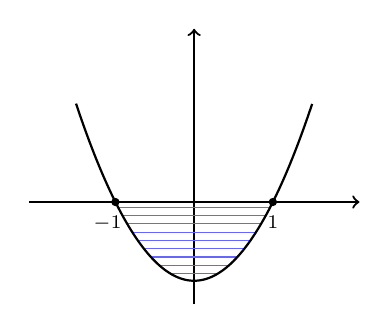
\begin{tikzpicture}

    \draw[->, thick] (-2.1,0) -- (2.1,0);
    \draw[->, thick] (0,-1.3) -- (0,2.2);

    \fill[
        pattern=horizontal lines,
        pattern color=blue!60
    ]
        (-1,0)
        -- plot[domain=-1:1, samples=100] (\x,{\x*\x-1})
        -- cycle;

    \draw[thick, domain=-1.5:1.5, samples=100]
        plot (\x,{\x*\x-1});

    \fill (-1,0) circle (1.5pt);
    \fill (1,0) circle (1.5pt);

    \node[below, font=\scriptsize] at (-1.1,-0.06) {$-1$};
    \node[below, font=\scriptsize] at (1,-0.06) {$1$};

    \end{tikzpicture}
\end{center}

\section{Funcions}

Definim una funció $f$ una \textbf{aplicació} i es defineix com;

\[f: A \rightarrow B\]
\[a \rightarrow f(a)\]

Que vol dir \textit{prenem un input a al conjunt A i li assignem un output f(a) que pertany al conjunt B}

Diem que una funció és injectiva quan una \textbf{sola imatge té un valor associat} ($x^2$ no ho és, $3x+2$ ho és)

En aquesta assignatura prenem funcións de $\R \rightarrow \R$ ja que són funcions en 2D i no toquem $\R^3$. Ara bé, no totes les funcións funcionen $\forall x \in \R$, si prenem la funció $f: \frac{1}{x}$ i la passem de $\R \rightarrow \R$ obtenim el conjunt input = $\{-\infty, \dots, 0, \dots, \infty\}$ peró en el output no hi ha cap numero que multiplicat per zero dongui 1 per tant per $x = 0$ la \textbf{funció es trenca}. De manera que hem de \textit{definir un conjunt D que s'anomena \textbf{domini de la funció}} on pertanyen tots els valors als que s'hi associa un valor.

\[f: D \rightarrow \R\]
\[x \rightarrow f(x)\]

Anomenem al conjunt $f(D)$ al conjunt de \textbf{totes les imatges de la funció} = \textbf{recorregut de la funció}.
\subsection{Tipus de Funcions}

Existeixen unes \textbf{funcions elementals a partir de les quals es construeix tot el càlcul}.

\begin{itemize}
    \item \textit{F. Lineals} $D = \R$, $f(x) = a+bx$
    \item \textit{Polinomis} $f(x) = x^n$ on $n \in \Z$
    \item \textit{Potències Enteres} $p(x) a_0 + a_1x^1 + \dots a_nx^n$ on $n\geq 0$
    \item \textit{Racionals} $f(x) = \frac{p(x)}{q(x)}$ on $q(x) \neq 0$
    \item \textit{Radicals} $f(x) = \sqrt[n]{x} = x^{\frac{1}{n}}$ on si $n \in \text{Parell } Dom(f) = R^+$
    \item \textit{Exponencials} $f(x) = a^x$ on $a > 0, x\in\{n,0,-n,\frac{1}{n}\} \forall n \in \Z$
    Aquestes ens donen un \textbf{creixement o decreixement exponencial}, aquesta funció és injectiva i és el $\log(x)$, en aquesta funció s'apliquen totes les propietats exponencial.
    \begin{itemize}
        \item $a^n \cdot a^m = a^{n + m}$
        \item $(a^n)^m = a^{n\cdot m} = (a^m)^n$
        \item $a^0: a^0 \cdot a^n = a^{0+n} = a^n \therefore a^0 = 1$
        \item $a^{-n}: a^{-n} \cdot a^n = a^{n-n} = a^0 \therefore a^{-n} = \frac{1}{a^n}$ on $a\neq 0$
    \end{itemize} 
\end{itemize}

\subsection{Funció Inversa}

Només existeix una funció inversa $f\rightarrow f^{-1}$, si la funció $f$ \textbf{és injectiva} i definim $f^{-1}$;

\[f^{-1}: Img \rightarrow D\]
\[f(x) \rightarrow x\]

és a dir \textbf{desfà} l'operació d'una funció qualsevol, el procediment és simple;

\begin{demobox}
    Per trobar la funció d'inversa de $f(x) = 3x + 5$, fem servir 4 passos;

    \begin{itemize}
        \item $f(x) = y(x)$
        \item Busquem ($x(y)$)
        \item $x=y$
        \item $x(y) = f^{-1}(x)$
    \end{itemize}

    \begin{align*}
        y &= 3x + 5\\
        x &= \frac{y-5}{3}\\
        y &= \frac{x-5}{3}\\
        f^{-1}(x) &= \frac{x-5}{3}  
    \end{align*}
\end{demobox}

Si hi ha alguna funció injectiva i \textbf{volem conèixer la inversa} reduïm el domini. Per exemple, definim $f(x)=x^2$ per $x>0$, la inversa $f^{-1}(x) = + \sqrt{x}$

\end{document}